\problemname{Morötter}
Tor och hans mor älskar morötter.
Varje dag ställer de fram en skål med 40 morötter och äter sedan morötter oavbrutet tills skålen är tom.
Om de båda är redo att ta en morot när det bara finns en kvar, så tar ingen av dem den sista.

\begin{figure}[h]
    \centering
  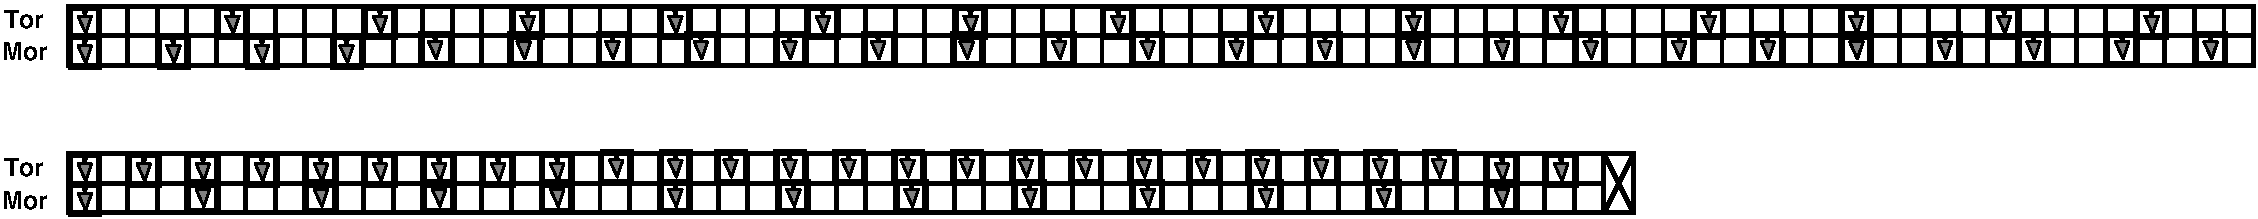
\includegraphics[width=1.0\textwidth]{morot.pdf}
\caption{Tidsschema för morotsätningen i exempel 1 (överst) och exempel 2 (underst). I det andra exemplet kommer ingen att ta den sista moroten.}
\end{figure}

Skriv ett program som, givet antal sekunder det tar för Tor respektive hans mor att äta varje morot (båda heltal), beräknar hur många morötter var och en får.

\section*{Indata}
Den första och enda raden består av två heltal $T$ och $M$ ($1 \le T, M \le ?$), tiden det tar för Tor respektive hans mor att äta en morot, i sekunder.

\section*{Utdata}
Skriv ut en rad med två heltal: först antalet morötter Tor äter, följt av antalet morötter hans mor äter.

\section*{Poängsättning}
Din lösning kommer att testas på en mängd testfallsgrupper.
För att få poäng för en grupp så måste du klara alla testfall i gruppen.

\noindent
\begin{tabular}{| l | l | p{12cm} |}
  \hline
  \textbf{Grupp} & \textbf{Poäng} & \textbf{Gränser} \\ \hline
  $1$    & $?$      & ? \\ \hline
  $2$    & $?$      & Inga ytterligare begränsningar. \\ \hline
\end{tabular}
